\documentclass{beamer}
\usetheme{Madrid}
% Abilita il supporto alle immagini
\usepackage{graphicx}
%Path relative to the main .tex file 
\graphicspath{ {./images/} }
\usepackage{fancybox}
\setbeamertemplate{navigation symbols}{}

% Informazioni da includere nella pagina del titolo:
\title[DCC performance in IEEE 802.11p] % opzionale
{On the performance of Decentralized Congestion Control in a real IEEE 802.11p testbed}

\fontsize{11}{13}\selectfont \author{\textbf{Studente: Antonio Solida - 178507}}

\institute[] % opzionale
{
    \fontsize{11}{13}\selectfont \textbf{Relatore: Prof. Carlo Augusto Grazia}
    \and
    Esame di Automotive Connectivity\\
    Corso di Laurea Magistrale in Ingegneria Informatica\\
    Percorso "\textit{Cloud \& Cybersecurity}"
    \and
    Dipartimento di Ingegneria "Enzo Ferrari"\\
    Università degli studi di Modena e Reggio Emilia
}

\date[17 ottobre 2024] % opzionale
{Modena, 17 ottobre 2024}

\begin{document}

\frame{\titlepage}

\begin{frame}
    \frametitle{Introduzione}
    \centering
    \begin{block}{Keywords}
        \begin{itemize}
            \item Reti \textbf{VANET} (\textit{Vehicular Ad-Hoc Networks}) \& \textbf{DSRC} (\textit{Dedicated Short-Range Communication})
            \item IEEE \textbf{802.11p} \& ETSI \textbf{ITS} (\textit{Intelligent Transport System})
            \item \textbf{CAM} (\textit{Community Awareness Message})
        \end{itemize}
    \end{block}
    
    \begin{columns}
        \begin{column}{0.5\textwidth}
            \centering
            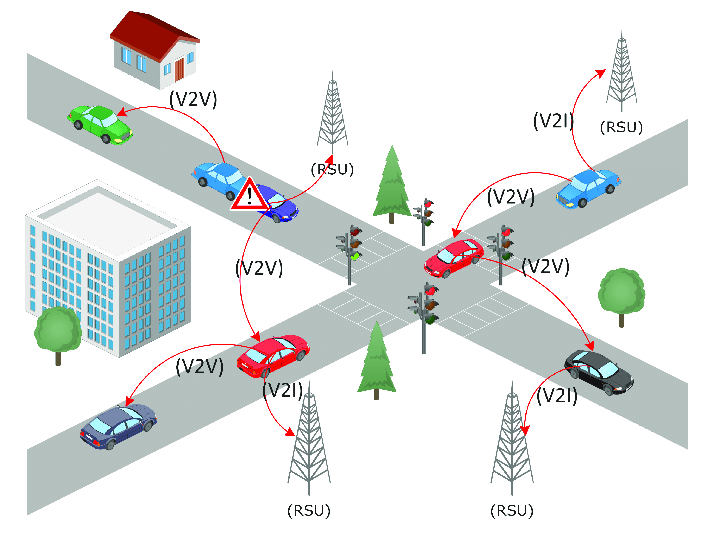
\includegraphics[width=1\textwidth]{vanet.png}
            \label{fig:vanet}
        \end{column}
        \begin{column}{0.5\textwidth}
            \centering
            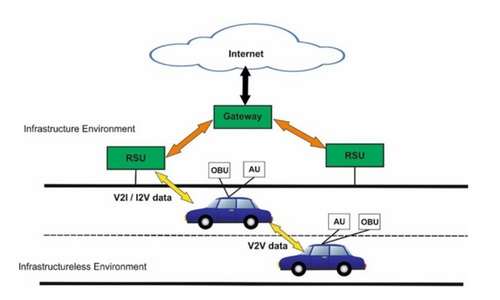
\includegraphics[width=1\textwidth]{routing_vanet.jpeg}
            \label{fig:obu_rsu}
        \end{column}
    \end{columns}
\end{frame}    

\begin{frame}
    \frametitle{Problema: congestione del canale}
    In ambienti con più veicoli, come una strada trafficata, l'accumulo di informazioni trasmesse può portare a una \alert{seria congestione del canale}, compromettendo la comunicazione.
    \vfill
    \begin{block}{Possibili cause}
        \begin{itemize}
            \vspace{5pt}
            \item {CAM inviati periodicamente}
            \vspace{5pt}
            \item {Invio di DENM}
            \vspace{5pt}
            \item {Altre trasmissioni sulla stessa banda}
            \vspace{5pt}
        \end{itemize}
    \end{block}
    
\end{frame}

\begin{frame}
    \frametitle{Soluzione: DCC con Transmit queues?}
    \centering
    \vfill
    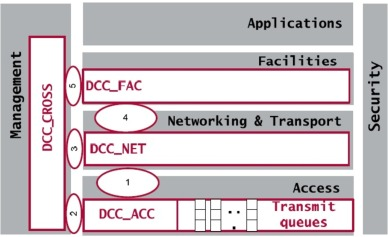
\includegraphics[width=0.5\textwidth]{dcc_edca.jpg}
    \vfill
    \begin{itemize}
        \item \textbf{Decentralized Congestion Control (DCC)}
        \vspace{15pt}
        \item \textbf{Classificazione del Traffico}
    \end{itemize}
    \vfill
\end{frame}

\begin{frame}
    \frametitle{Descrizione testbed}
    \centering
    \begin{minipage}{0.58\textwidth}
        % Aggiunta dell'immagine del diagramma
        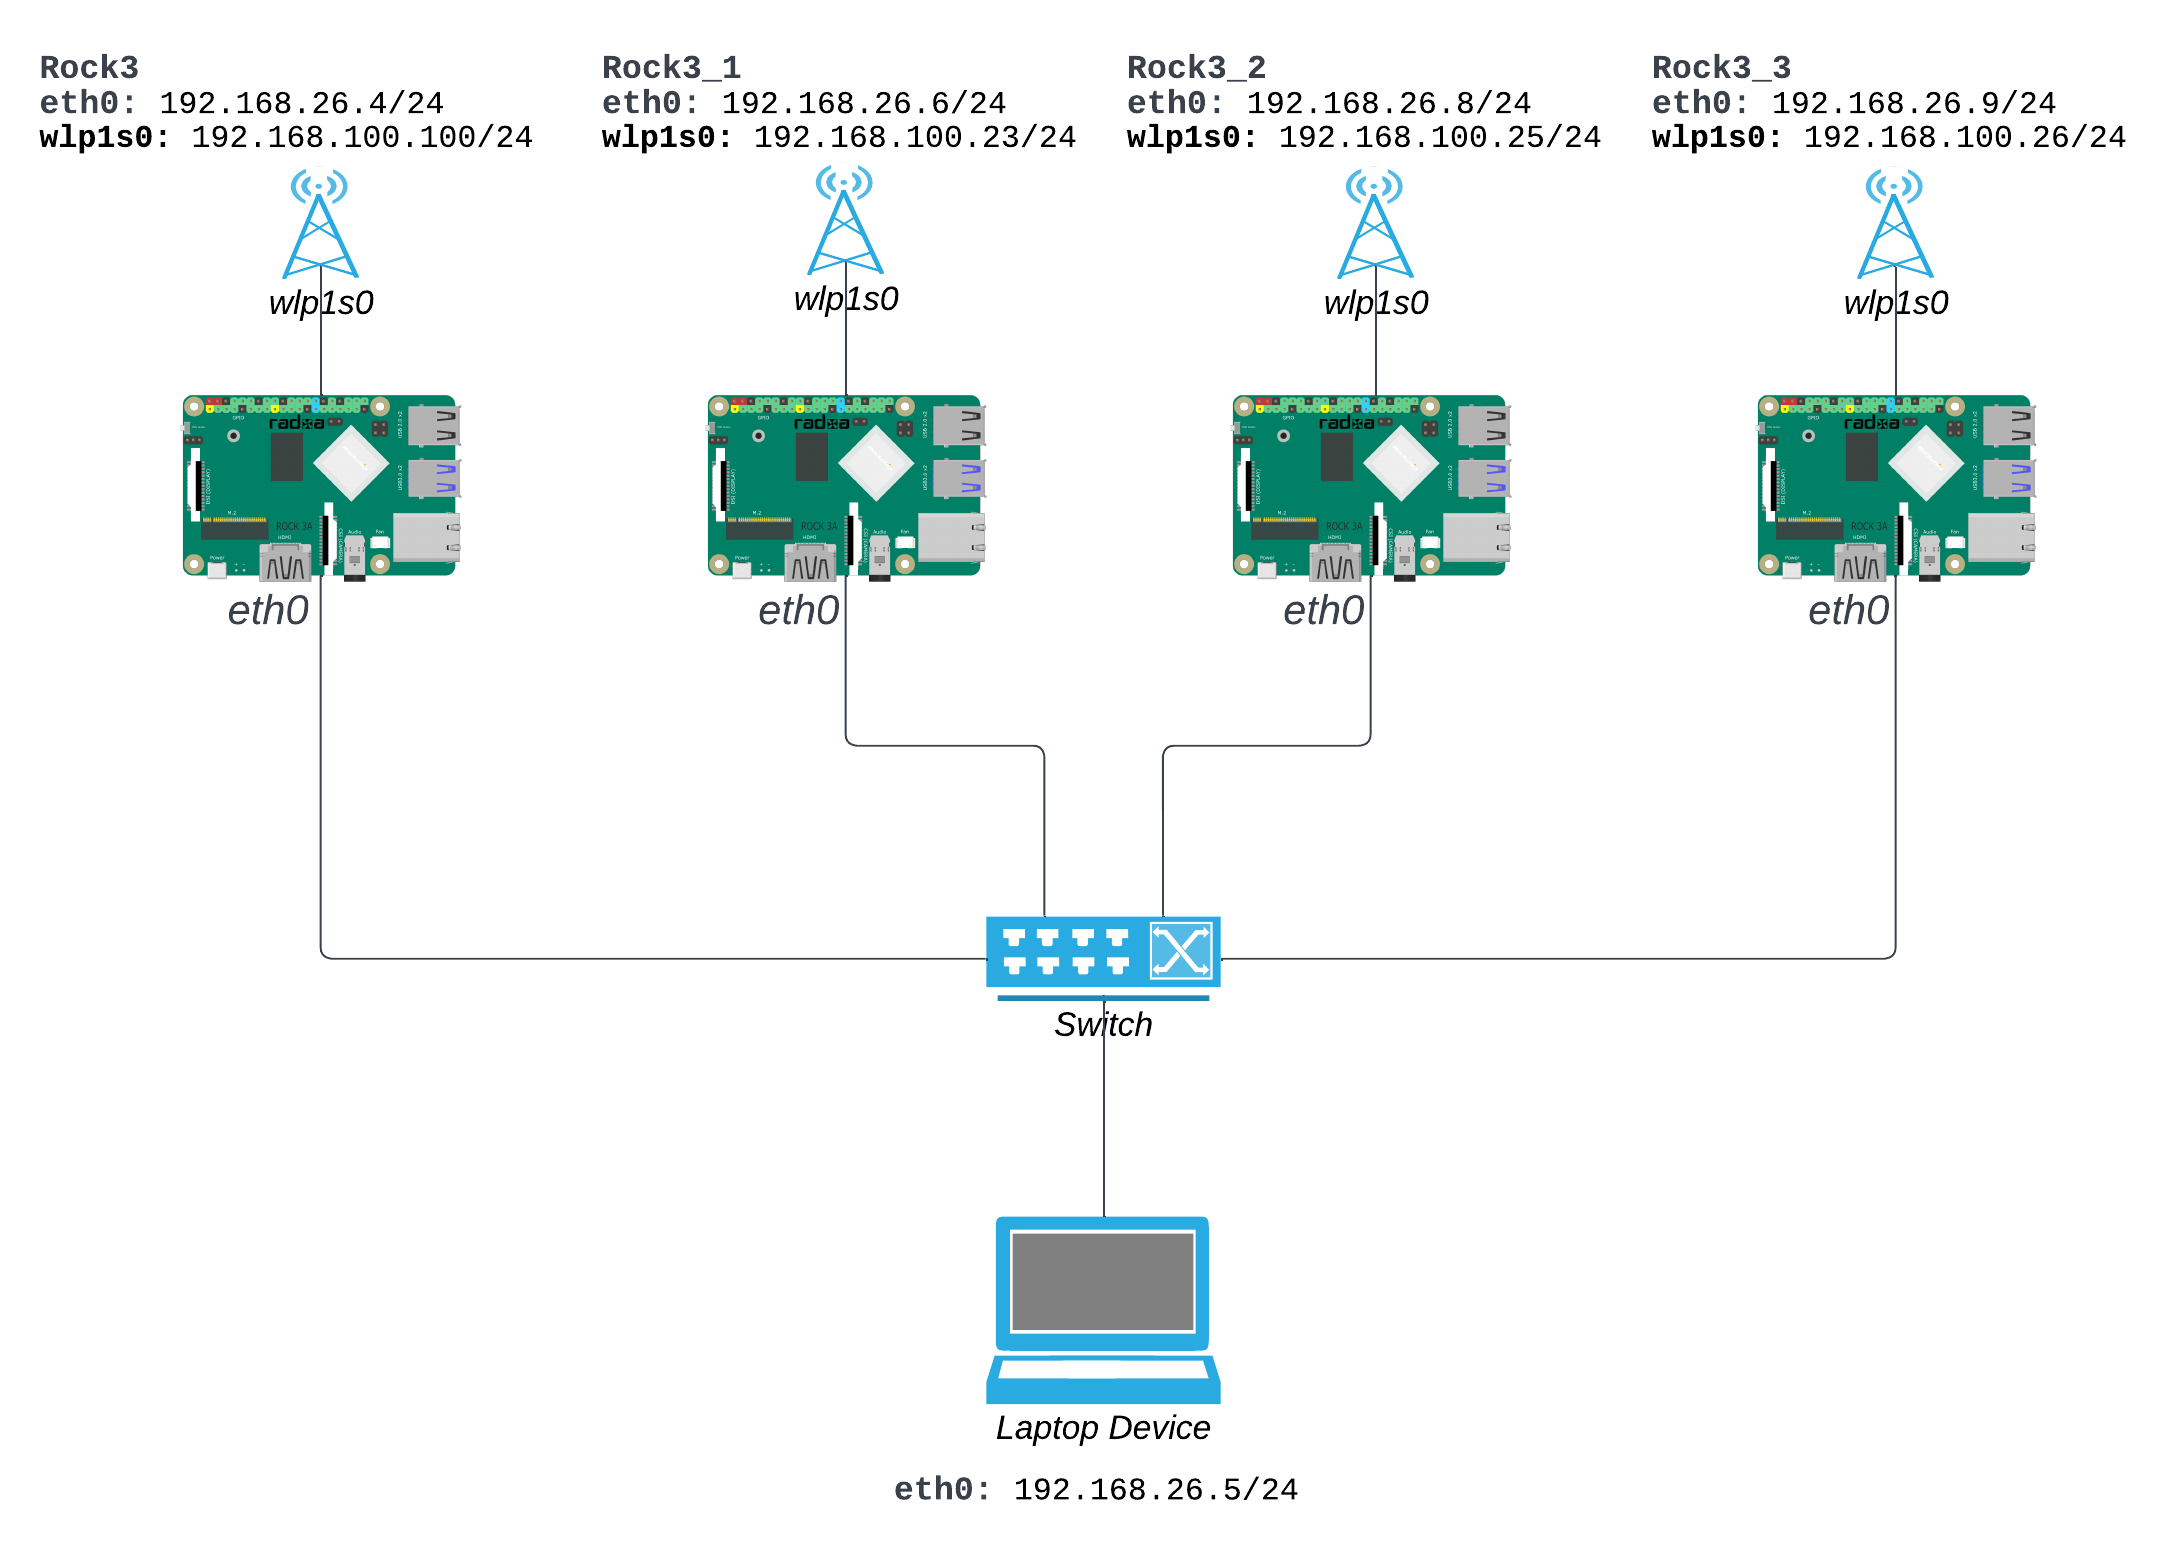
\includegraphics[width=\textwidth]{topology.png}
    \end{minipage}%
    \hfill
    \begin{minipage}{0.38\textwidth}
        \centering
        % Immagine della scheda Rock 3A
        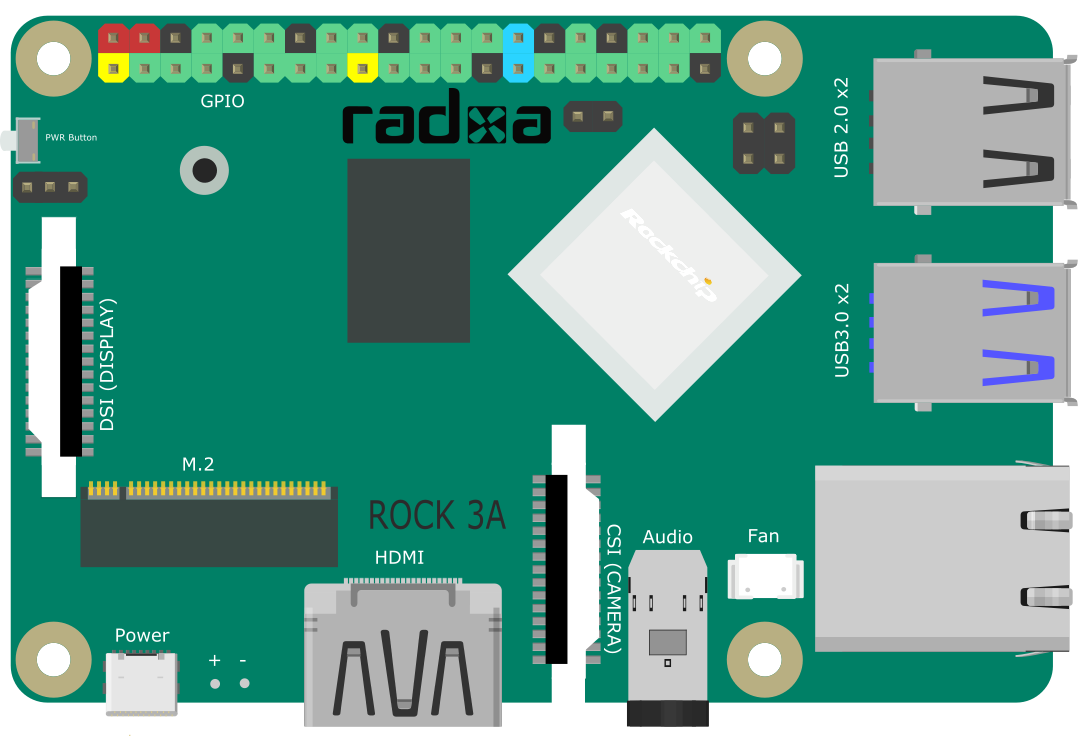
\includegraphics[width=\textwidth]{ROCK_3A.png}
        \vspace{0.5cm}
        % Immagine del laptop
        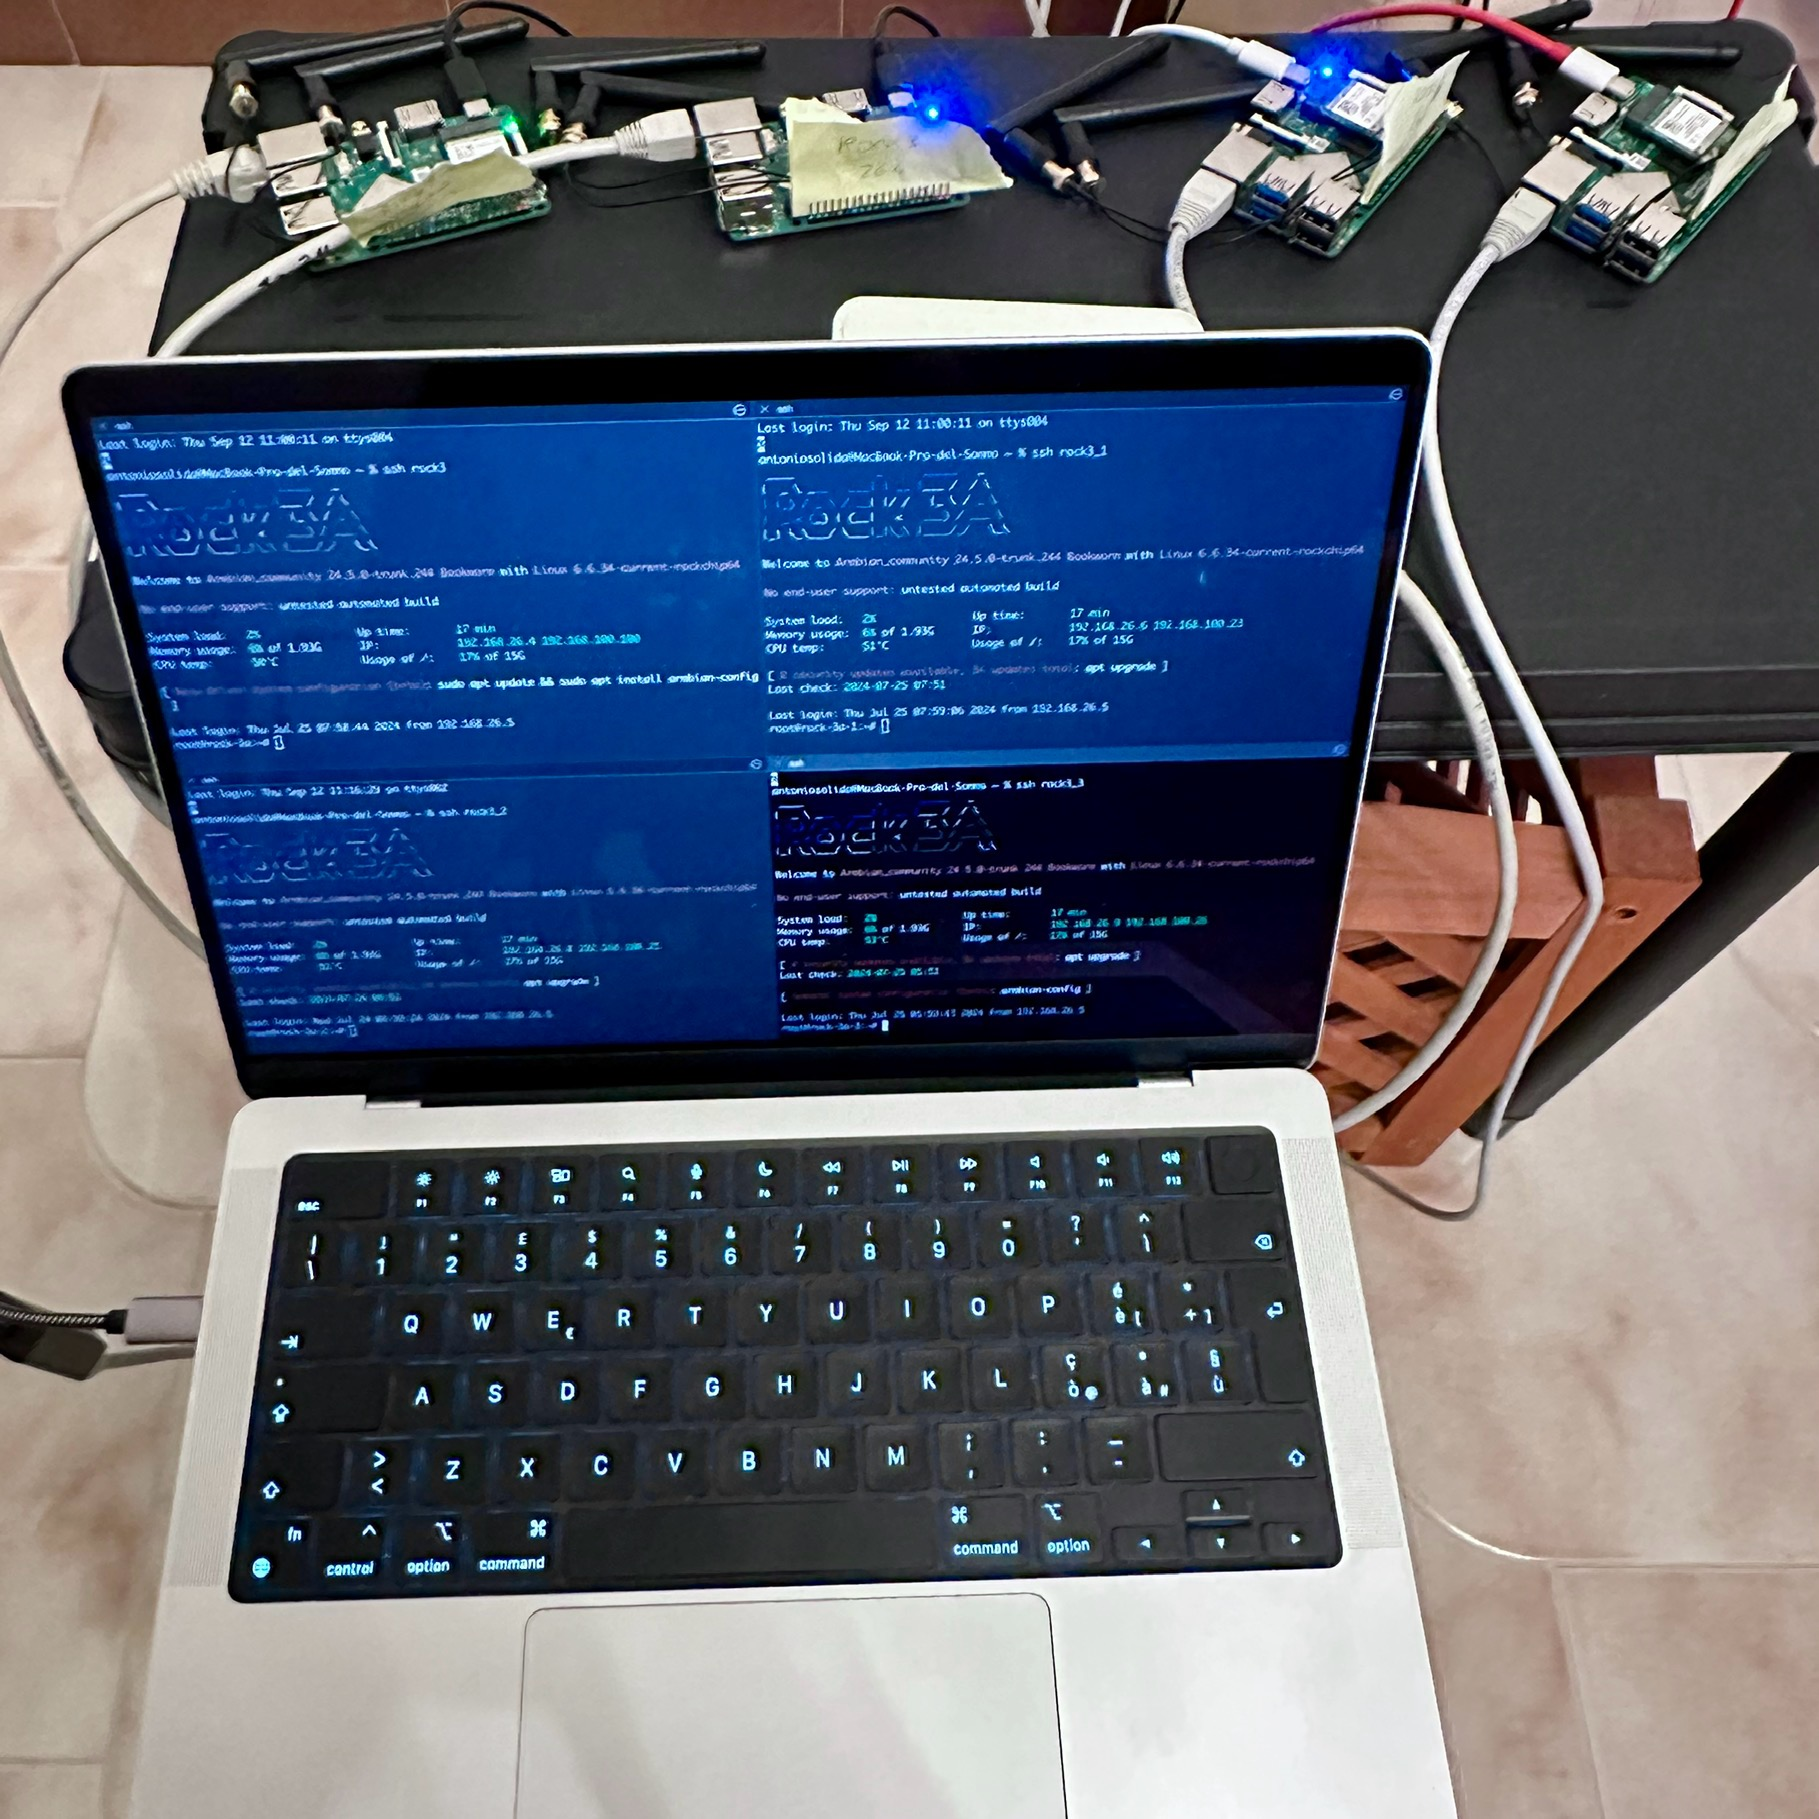
\includegraphics[width=\textwidth]{topology_photo.jpg}
    \end{minipage}
\end{frame}

\begin{frame}
    \frametitle{Test performance flussi TCP}
    \vfill
    \centering
    Dispositivi suddivisi in due gruppi:
    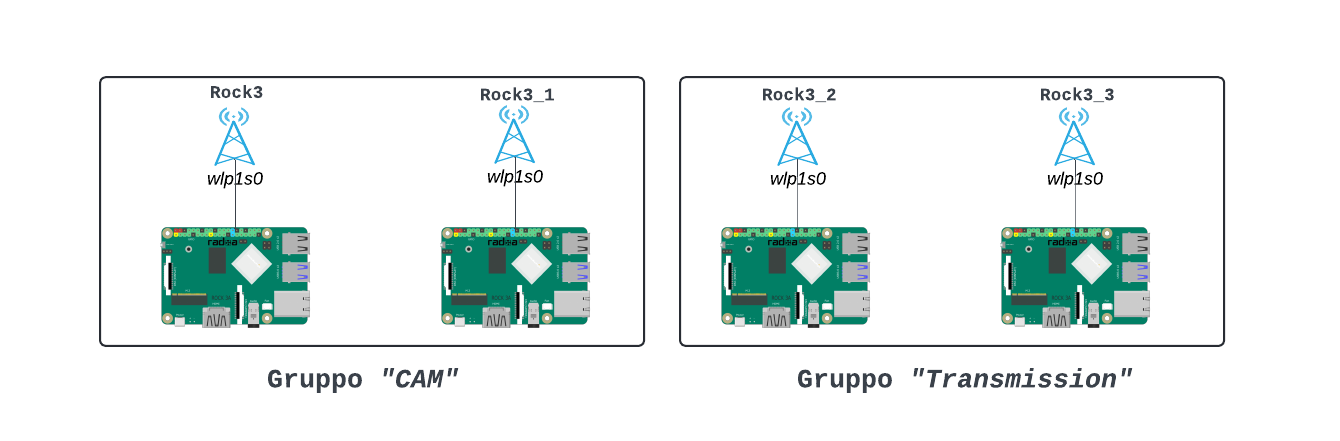
\includegraphics[width=0.7\textwidth]{Rock scheme.png}
    \begin{itemize}
        \item \textit{Gruppo "CAM"}: due dispositivi che creano congestione (ove previsto).
        \item \textit{Gruppo "Transmission"}: due dispositivi per la trasmissione delle informazioni.
    \end{itemize}
    \vfill
\end{frame}

\begin{frame}
    \frametitle{Trasmissione in ambiente non congestionato}
    
    \begin{minipage}{0.45\textwidth}
        \textbf{Quality of Service assente}\\
        \textit{Throughput medio Stream ID 1}: 3.49 Mbps\\
        \textit{Throughput medio Stream ID 2}: 3.47 Mbps\\
        \vspace{1cm}
        
        \textbf{Quality of Service presente}\\
        \textit{Throughput medio Stream ID 1 (AC\_VO)}: 7.96 Mbps\\
        \textit{Throughput medio Stream ID 2 (AC\_BK)}: 0.61 Mbps\\
    \end{minipage}
    \hfill
    \begin{minipage}{0.5\textwidth}
        \centering
        \begin{minipage}{\textwidth}
            % Primo grafico (Quality of Service assente)
            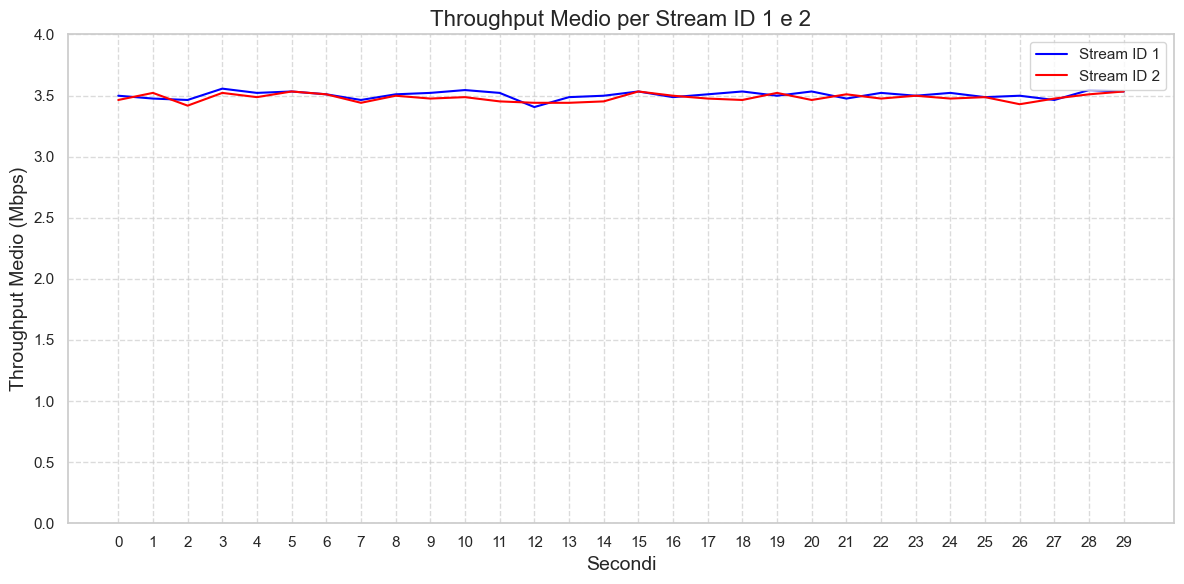
\includegraphics[width=\textwidth]{t1_c0_main.png}
            \vspace{0.5cm}
        \end{minipage}
        \begin{minipage}{\textwidth}
            % Secondo grafico (Quality of Service presente)
            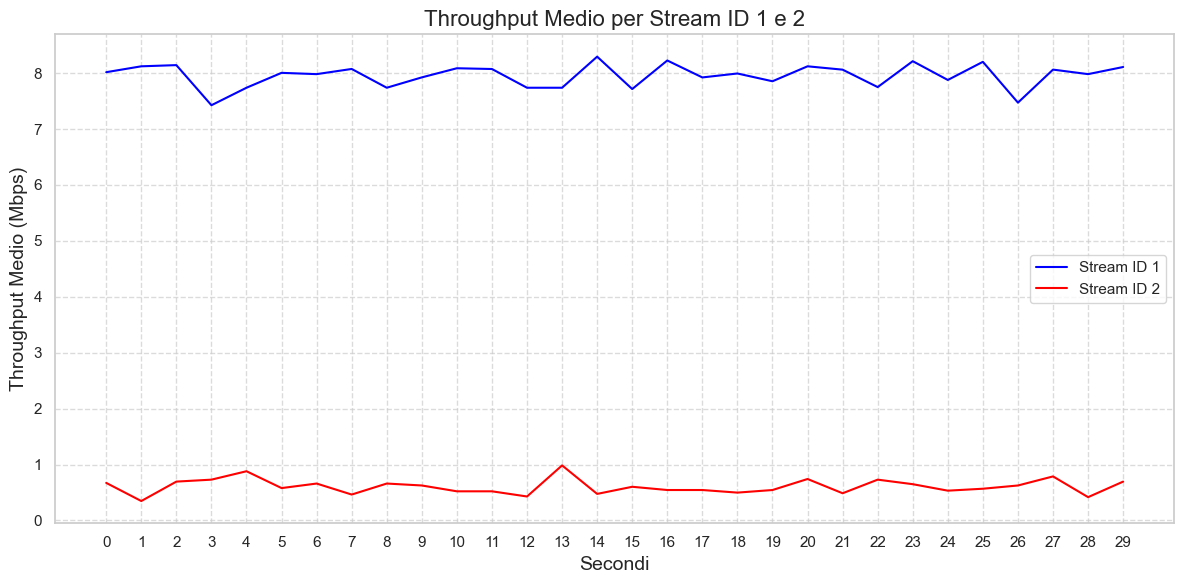
\includegraphics[width=\textwidth]{t2_c0_main.png}
        \end{minipage}
    \end{minipage}

\end{frame}


\begin{frame}
    \frametitle{Trasmissione in ambiente parzialmente congestionato}
    
    \begin{minipage}{0.45\textwidth}
        % Quality of Service assente
        \textbf{Quality of Service assente}\\
        \textit{Throughput medio Stream ID 1}: 3.13 Mbps\\
        \textit{Throughput medio Stream ID 2}: 3.13 Mbps\\
        
        \vspace{1cm}
        
        % Quality of Service presente
        \textbf{Quality of Service presente}\\
        \textit{Throughput medio Stream ID 1 (AC\_VO)}: 6.73 Mbps\\
        \textit{Throughput medio Stream ID 2 (AC\_BK)}: 0.77 Mbps\\
    \end{minipage}
    \hfill
    \begin{minipage}{0.5\textwidth}
        \centering
        \begin{minipage}{\textwidth}
            % Primo grafico (Quality of Service assente)
            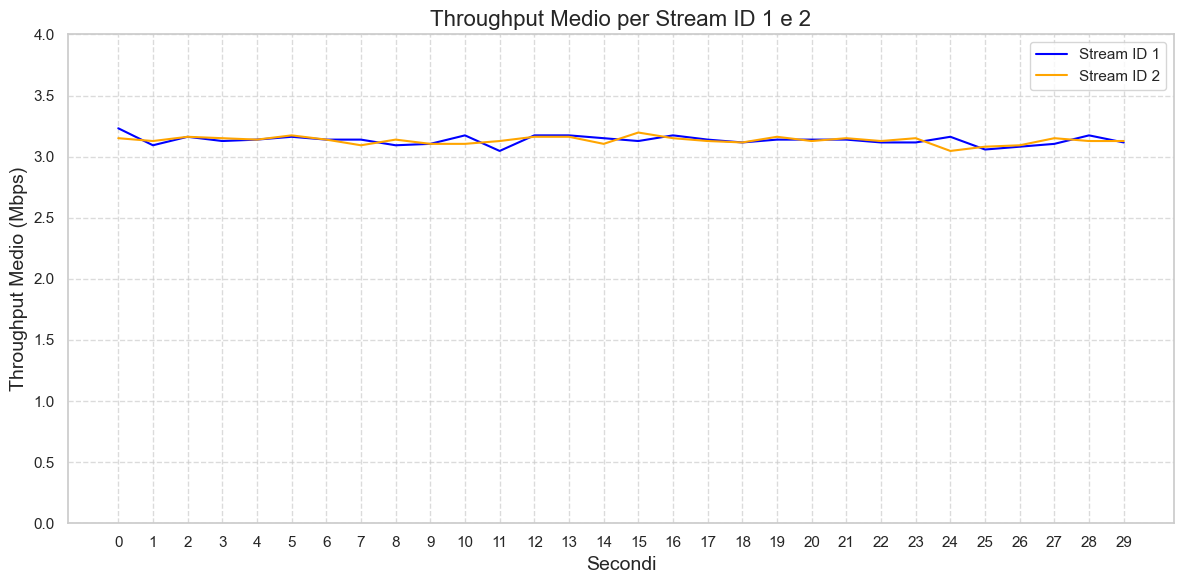
\includegraphics[width=\textwidth]{t1_c1_main.png}
            \vspace{0.5cm}
        \end{minipage}
        \begin{minipage}{\textwidth}
            % Secondo grafico (Quality of Service presente)
            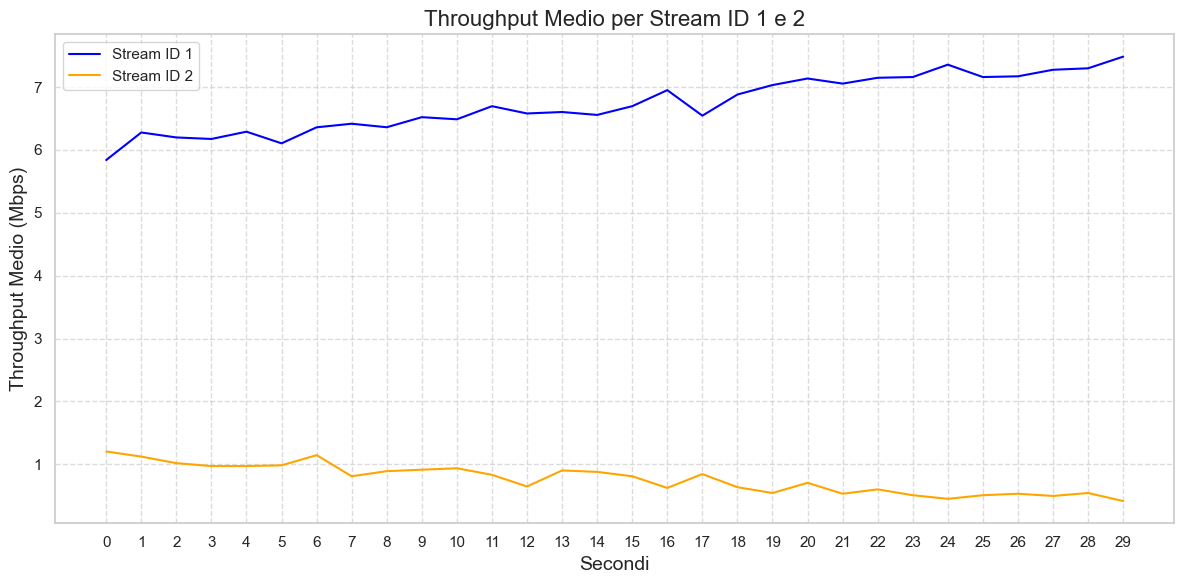
\includegraphics[width=\textwidth]{t2_c1_main.png}
        \end{minipage}
    \end{minipage}

\end{frame}

\begin{frame}
    \frametitle{Trasmissione in ambiente totalmente congestionato}
    
    \begin{minipage}{0.45\textwidth}
        % Quality of Service assente
        \textbf{Quality of Service assente}\\
        \textit{Throughput medio Stream ID 1}: 1.14 Mbps\\
        \textit{Throughput medio Stream ID 2}: 1.19 Mbps\\
        
        \vspace{1cm}
        
        % Quality of Service presente
        \textbf{Quality of Service presente}\\
        \textit{Throughput medio Stream ID 1 (AC\_VO)}: 6.19 Mbps\\
        \textit{Throughput medio Stream ID 2 (AC\_BK)}: 0.30 Mbps\\
    \end{minipage}
    \hfill
    \begin{minipage}{0.5\textwidth}
        \centering
        \begin{minipage}{\textwidth}
            % Primo grafico (Quality of Service assente)
            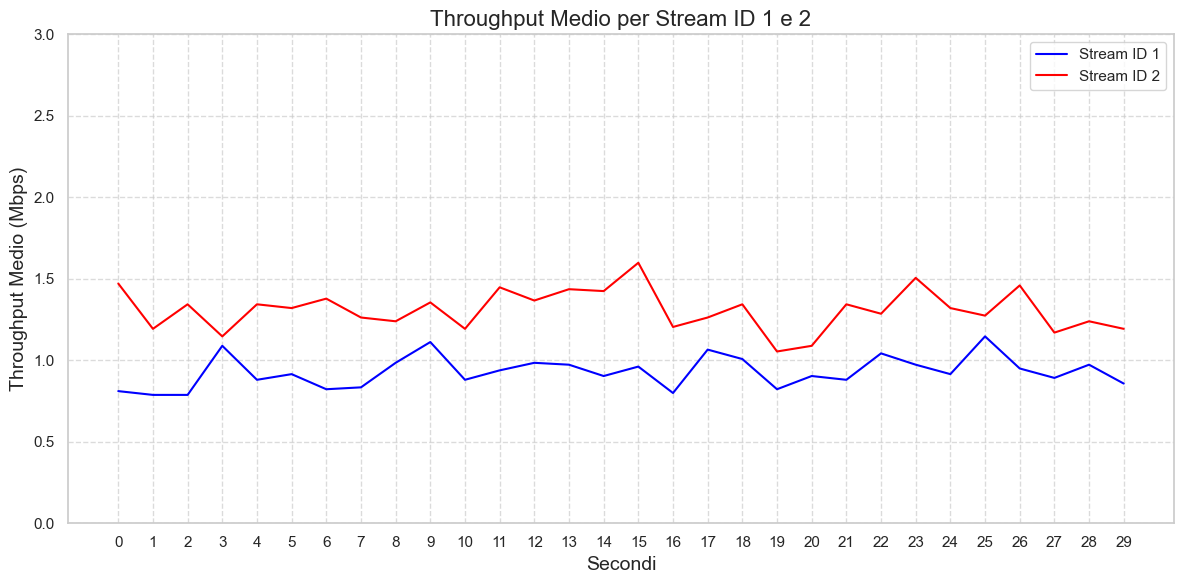
\includegraphics[width=\textwidth]{t1_c2_main.png}
            \vspace{0.5cm}
        \end{minipage}
        \begin{minipage}{\textwidth}
            % Secondo grafico (Quality of Service presente)
            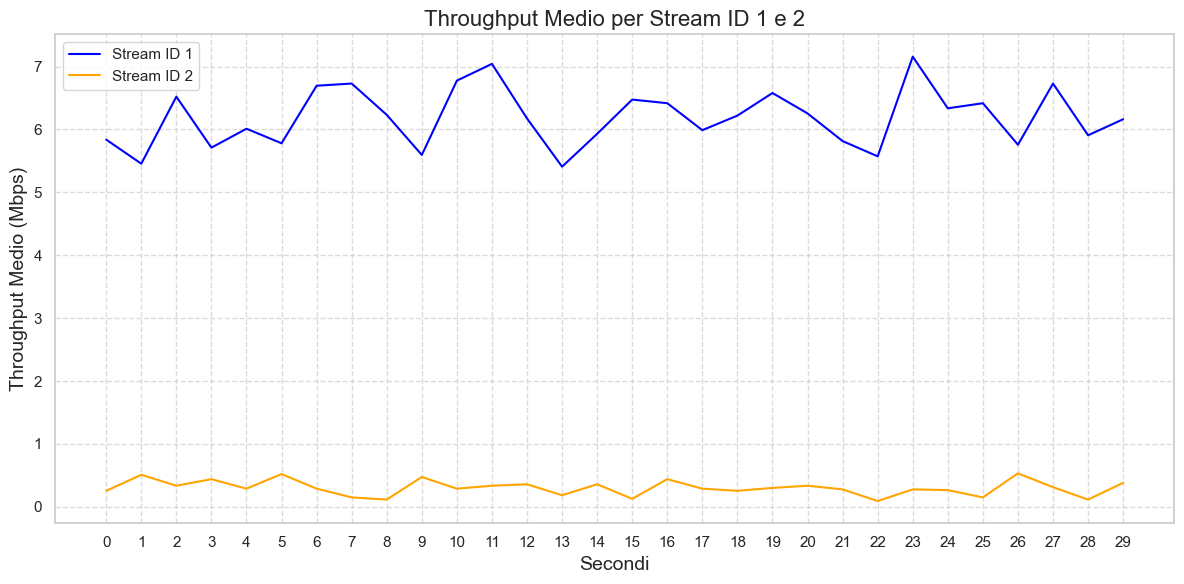
\includegraphics[width=\textwidth]{t2_c2_main.png}
        \end{minipage}
    \end{minipage}

\end{frame}


\begin{frame}
    \frametitle{Considerazioni}
    \centering
    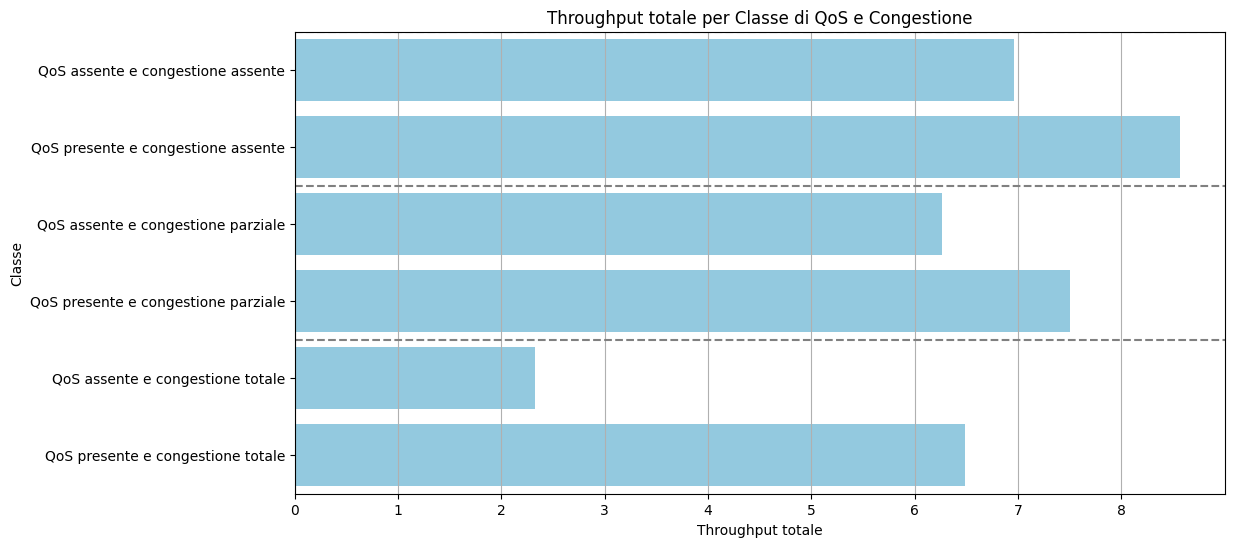
\includegraphics[width=0.9\textwidth]{throughput_bar.png}
    \begin{block}{Risultati riscontrati}
        \begin{itemize}
            \item Maggior throughput nel flusso a priorità maggiore.
            \item Maggiore efficienza nello sfruttamento della banda.
        \end{itemize}
    \end{block}
\end{frame}

\begin{frame}
    \frametitle{Conclusioni finali}

    \begin{enumerate}
        \item \textbf{Saturazione del Canale:} In assenza di meccanismi di gestione, il numero crescente di dispositivi può saturare il canale, riducendo la qualità del servizio, soprattutto in scenari urbani.

        \item \textbf{Classi di Priorità:} Implementazione di classi di priorità per i messaggi trasmessi, migliorando l'uso delle risorse di rete e garantendo banda per comunicazioni critiche.

        \item \textbf{Risultati Sperimentali:} L'adozione di code di priorità ha dimostrato di aumentare significativamente la disponibilità di banda e ridurre i tempi di attesa per messaggi critici.

        \item \textbf{Implicazioni Future:} Necessità di valutare l'integrazione di datarate più elevati e modulazioni più efficienti per migliorare le performance di rete.
    \end{enumerate}

\end{frame}

\begin{frame}
    \frametitle{Grazie per l'attenzione!}

    \begin{center}
        \textbf{Grazie per l'attenzione!} \\[1em]
        A disposizione per eventuali domande e dubbi.
    \end{center}

\end{frame}

\end{document}
